
\subsection{Locating Errors with Witnesses}
\label{sec:locating}

We have seen that \toolname can effectively synthesize witnesses to
explain the majority of (novice) type errors, but a good error report
should also help \emph{locate} the source of the error.
%
Thus, our final experiment seeks to use \toolname's witnesses as
localizations.


As discussed in \S~\ref{sec:methodology}, we recorded
each interaction of our students with the \ocaml top-level system.
%
In addition to collecting ill-typed programs, we collected
subsequent, fixed versions of the programs.
%
For each ill-typed program in a student's interaction trace, we identify
the student's fix by searching for the first type-correct program
that follows it in the trace.
%
We then use an expression-level \emph{diff}~\cite{Lempsink2009-xf} to
determine which sub-expressions changed between the ill-typed program
and the student's fix, and treat those expressions as the source of the
type error.

Not all ill-typed programs will have an associated fix; furthermore,
at some point a ``fix'' becomes a ``rewrite''.
%
We do not wish to consider the ``rewrites'', so we discard outliers
where the fraction of expressions that have changed is more than one
standard deviation above the mean, establishing a diff threshold of
45\%.
%
This accounts for roughly 14\% of programs pairs we discovered, leaving
us with 2,425 program pairs.

For each pair of an ill-typed program and its fix, we run \toolname and
collect two sets of source locations:
%
(1) the source location corresponding to the stuck term; and
%
(2) the source locations that \emph{produced} the values inside the
stuck term.
%
Intuitively, these two classes of locations correspond to \emph{sinks}
and \emph{sources} for typing constraints.
%
For example, in the @sqsum@ program from \S~\ref{sec:advantage-traces}
the stuck term is \verb!0 @ 1!.
%
This corresponds to the call to \verb!@! on line 3, and contains
the literal @0@ from line 2 and the value @1@ produced by the
@*@ on line 3.

We compare \toolname's witness-based predictions against a baseline of
the \ocaml compiler as well as the state-of-the-art %type error
localization tools \sherrloc and \mycroft.
%
\sherrloc~\cite{Zhang2014-lv} attempts to predict the most likely source
of a type error by searching the typing constraint graph for constraints
that participate in many unsatisfiable paths and few satisfiable paths.
%
\mycroft~\cite{Loncaric2016-uk} reduces the localization problem to
MaxSAT by searching for a minimal subset of constraints that can be
removed, such that the resulting system is satisfiable.
%
Both tools produce a \emph{set} of equally-likely expressions to blame
for the error (in practice the set contains only a few expressions),
similar to \toolname's witness-based predictions.

We evaluate each tool based on whether \emph{any} of its predictions
identifies a changed expression.
%
There were a number of student programs where \mycroft or \sherrloc
encountered an unsupported language feature or timed out after one
minute, or where \toolname failed to produce a witness.
%
We discard all such programs in our evaluation to level the playing
field, around 15\% for each tool, leaving us with a benchmark set of
1,569 programs.

\paragraph{Threats to Validity}
Our benchmarks were drawn from students in an undergraduate course
at \ucsdbench\ and may not be representative of other student bodies.
%
We mitigate this threat with a large empirical evaluation of 1,569
programs, drawn from a cohort of 46 students.
%
A similar threat is that students are not industrial programmers, thus
our results may not translate to large-scale software engineering.
%
In particular, \toolname's reliance on running the program suggests that
scaling it to larger programs would be more difficult than static
methods.
%
However, in our experience programmers are able to construct a mental
model of type systems after sufficient exposure, at which point
traditional error reports may suffice.
%
We are thus particularly interested in aiding novice programmers as
they learn to work with the type system.

Our definition of the next well-typed program as the intended ground
truth answer is another threat to validity. Students might submit
multiple well-typed ``rewrites'' between the initial ill-typed program
and the final intended answer.
%
Our approach to discarding outliers is intended to mitigate this threat.
%
A similar threat is our removal of programs where any of the tools could
not produce an answer.
%
It may be, for example, that \mycroft and \sherrloc are particularly
effective on programs that do not admit dynamic witnesses.
%
Finally, our use of student fixes as oracles for the source of type
errors assumes that students are able to correctly identify the source.
%
As the students are in the process of learning \ocaml and the type
system, this assumption may be faulty, \emph{expert} users may disagree
with the student fixes.
%
We believe, however, that it is reasonable to use student fixes as
oracles, as the student is the best judge of what she \emph{intended} to
do.

\begin{figure}[t]
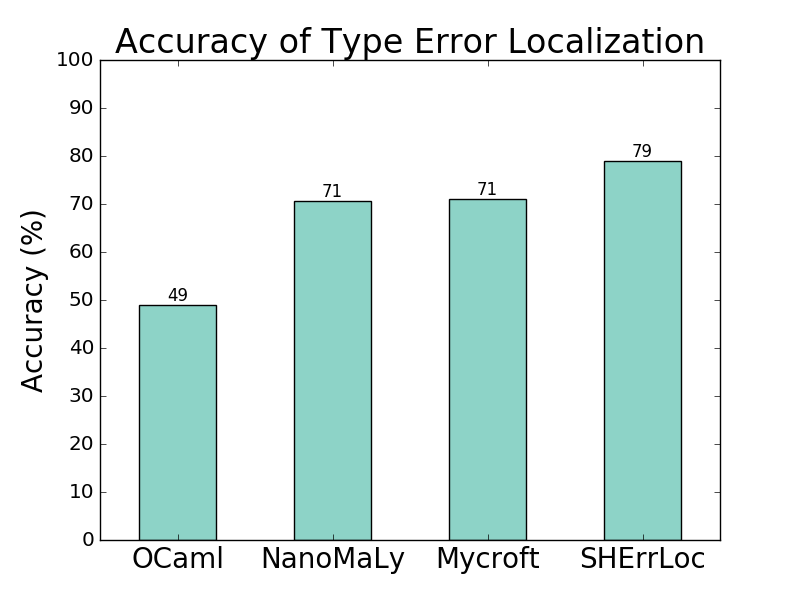
\includegraphics[width=0.7\linewidth]{blame.png}
\caption{Accuracy of type error localization. \toolname's witness-based
  predictions outperform \ocaml by 22 points, and are competitive
  with the state-of-the-art tools \mycroft and \sherrloc.}
\label{fig:results-blame}
\end{figure}

\paragraph{Results}
Figure~\ref{fig:results-blame} summarizes our results, which show that
\toolname's witnesses are competitive with \mycroft and \sherrloc in
automatically locating the source of a type error.
%
\toolname, \mycroft, and \sherrloc all outperform the \ocaml compiler,
which is not surprising given that they can produce multiple possible
error locations, while the \ocaml compiler is limited to one predicted
error location.
%
Interestingly, while all tools have a median of 2 predicted error
locations per program, \mycroft and \sherrloc have a long tail with a
maximum of 22 (\resp 12) locations, while \toolname's maximum is 5
locations.
%
We also note that while \mycroft and \sherrloc were designed
specifically to \emph{localize} type errors, \toolname's foremost
purpose is to \emph{explain} them, we consider its ability to localize
type errors an added benefit.

%%% Local Variables:
%%% mode: latex
%%% TeX-master: "main"
%%% End:
